%%% DOCUMENTCLASS 
%%%-------------------------------------------------------------------------------

\documentclass[a4paper,11pt, onecolumn, openany]{memoir}

%%% PACKAGES 
%%%------------------------------------------------------------------------------

% Język i czcionki
\usepackage[utf8]{inputenc} % If utf8 encoding
% \usepackage[lantin1]{inputenc} % If not utf8 encoding, then this is probably the way to go
\usepackage[T1]{fontenc}
\usepackage{polski}
\usepackage[polish]{babel} 
\usepackage[final]{microtype} % Less badboxes
\usepackage{lmodern}
\usepackage{tgpagella}

% Bibliografia
\usepackage{natbib}

% \usepackage{kpfonts} %Font
% \usepackage{tikz} % Figures
\usepackage{graphicx} % Include figures
\usepackage{import}
\usepackage{tcolorbox}
\graphicspath{ {ilustracje/} }
\definecolor{titlepagecolor}{cmyk}{0.7,.30,0,.40}
\definecolor{miejscekolor}{cmyk}{0,0,1,.10}
\definecolor{code-gray}{gray}{0.95} 
%%% PAGE LAYOUT 
%%%------------------------------------------------------------------------------

\setlrmarginsandblock{0.15\paperwidth}{*}{1} % Left and right margin
\setulmarginsandblock{0.2\paperwidth}{*}{1}  % Upper and lower margin
\checkandfixthelayout


%%% INTERNAL HYPERLINKS
%%%-------------------------------------------------------------------------------

\usepackage{hyperref}   % Internal hyperlinks
\hypersetup{
	pdfborder={0 0 0},      % No borders around internal hyperlinks
	pdfauthor={Tomasz Nycz} % author
}
\usepackage{memhfixc}   %

%%% THE DOCUMENT
%%% Where all the important stuff is included!
%%%-------------------------------------------------------------------------------

\author{Tomasz Nycz}
\title{Formaty i relacje przestrzenne w QGIS}

\usepackage{lipsum} % Just to put in some text

\begin{document}
	
	\frontmatter
	
	\maketitle


\mainmatter
\part{Odniesienia przestrzenne}
	\chapter{Zbiory danych przestrzennych}
		\section{Wymagania prawne}
			\subsection{GML}
		\section{GeoPackage - następca Shapefile}
			\subsection{Tworzenie zbioru Geopackage}
			\subsection{Połączenie ze zbiorem}
		\section{Baza danych w GeoPackage}
			\subsection{Dodawanie wielu warstw}
			\subsection{Dołączanie projektu}
			\subsection{Dołączanie symboli i styli}		

	\chapter{Układy współrzędnych}
		\section{CRS i układ współrzędnych}
		W środowisku GIS możemy spotkać się z pojęciami CRS, odwzorowania kartograficznego, układu współrzędnych, oraz tzw. datum czy gridshift. Do dalszej komfortowej pracy konieczne jest zapoznanie się z nimi, oraz ich wzajemnymi powiązaniami.
		\begin{itemize}
			\item 		\textbf{Coordinate Reference System} - system odniesień przestrzennych. Jest to zbiór parametrów opisujących wszelkie cechy odniesień przestrzennych konieczne do poprawnego wskazania unikalnego miejsca w odniesieniu do powierzchni Ziemi. Należą do nich odwzorowanie kartograficzne, elipsoida, tzw. datum, południk i równoleżnik początkowy, oraz jednostki miary (stopnie, metry, sążnie, etc.)
			\item \textbf{Odwzorowanie kartograficzne} - jest to matematyczna realizacja sposobu odwzorowania elipsoidy obrotowej na płaszczyźnie mapy (lub zwizualizowania pseudo-trójwymiarowego w kartografii komputerowej). W praktyce europejskiej spotkamy się z odwzorowaniami: poprzecznym Merkatora, Gaussa-Kr\"{u}gera, azymutalnym Lamberta. W mapach obecnie archiwalnych popularne były również odwzorowania quasi-stereograficzne (WIG i GUGIK80) i Cassiniego-Soldnera. Można też było się spotkać z odwzorowaniami wielościennymi (np. wczesne edycje Messtichblatt).
			\item \textbf{Elipsoida} - to bryła powstała w wyniku obrotu elipsy wokół jej osi symetrii. Ziemię uznajemy w dużym uproszczeniu za elipsoidę obrotową (choć jej kształt jest dużo bardziej skomplikowany - nazywany geoidą). Ruch obrotowy Ziemi sprawia, że średnica równika jest o 43 km większa niż średnica pomiędzy biegunami. W czasach gdy kształt i rozmiary naszej planety były dopiero poznawane, powstało wiele opracowań opisujących parametry półosi wielkiej (a), półosi małej (b), oraz spłaszczenia (1/f). W naszych dalszych pracach będziemy wykorzystywać elipsoidy Bessela, Krassowskiego, oraz WGS84(GRS80).
			\item \textbf{Datum} - to geodezyjny układ odniesienia, opisujący kształt geoidy globalnie (np. systemy ETRS89/2000), jak również bardziej lokalnie (Pułkowo, Rauenberg, Hermannskogel). Obecnie w praktyce GIS geodezyjne układy odniesienia opisują translację względem geocentrycznego układu ETRF 89.
			\begin{figure}[!ht]
				\centering
				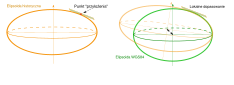
\includegraphics[width=15cm]{crs-transformacja-elipsoidy}
				\caption{Datum - Transformacja między układami odniesienia (za \citep{Affek_Georeferencing_2013})}
			\end{figure}
		    \item EPSG -  Rejestr i baza danych o układach odniesień (SRS i CRS), dawniej prowadzony przez \textbf{European Petroleum Survey Group}, obecnie Komitet Geomatyczny IOGP. Znajdują się w nim opisy parametrów elipsoid, południków zerowych, oraz całych CRS. Zamiennie z pojęciem kodu EPSG używa się terminu SRID - trochę szerszego, zawierającego również definicje własne producentów oprogramowania. Tabelę kodów EPSG przydatnych w codziennej pracy znajdziesz na końcu tego rozdziału. Można również skorzystać z wyszukiwarek kodu np. \hyperlink{https://epsg.org/search/map}{https://epsg.org/search/map}
		    \end{itemize}
	    Pozostałe parametry używane przy definiowaniu CRS opiszemy bezpośrednio przy stosowanych układach współrzędnych.
	
		\section{Uwarunkowania prawne}
		Wymagania prawne co do stosowanych układów odniesienia zdefiniowane są w rozporządzeniu Rady Ministrów z dnia 15 października 2012 r. w sprawie państwowego systemu odniesień przestrzennych (Dz.U. 2012 poz. 1247)\footnote{http://isap.sejm.gov.pl/isap.nsf/DocDetails.xsp?id=WDU20120001247}.
\begin{tcolorbox}[colback=black!5!white,colframe=white!55!black,title=§ 15. 1 i 2 rozporządzenia]
	§ 15. 1. Państwowy system odniesień przestrzennych stosuje się w pracach geodezyjnych i kartograficznych oraz przy
tworzeniu zbiorów danych przestrzennych przez organy władzy publicznej, przy czym:
\begin{enumerate}
	\item układ współrzędnych PL-LAEA stosuje się na potrzeby analiz przestrzennych i sprawozdawczości na poziomie ogólnoeuropejskim;
	\item układ współrzędnych PL-LCC stosuje się na potrzeby wydawania map w skali 1:500 000 i w mniejszych skalach;
	\item układ współrzędnych PL-UTM stosuje się na potrzeby wydawania standardowych opracowań kartograficznych w skalach od 1:10 000 do 1:250 000, wydawania map morskich oraz wydawania innych map przeznaczonych na potrzeby
	bezpieczeństwa i obronności państwa;
	\item układ współrzędnych PL-2000 stosuje się na potrzeby wykonywania map w skalach większych od 1:10 000 – w szczególności mapy ewidencyjnej i mapy zasadniczej.
\end{enumerate}
2. W pracach geodezyjnych i kartograficznych innych niż wymienione w ust. 1 pkt 1–4 stosuje się układ współrzędnych
PL-UTM lub układ współrzędnych PL-1992.
\end{tcolorbox}	
			\subsection{PL-1992}
			Układ (w dalszej części skryptu będziemy używać nazwy układ 92) oparty jest o odwzorowanie Gaussa-Kr\"ugera z południkiem osiowym 19E. Praktyczna stosowalność układu między 14E i 24.30E. Współrzędna wschodnia (X) na południku osiowym przyjmuje wartość 500000, zaś współrzędna północna -5300000. Zniekształcenie skali na południku osiowym przyjmuje wartość 0,9993 (co przekłada się na skurcz -0,7m/km).
			\subsection{PL-2000}
			Układ PL-2000 (dalej w skrócie będziemy nazywać go 2000, ze wskazaniem strefy), tak jak układ 92 oparty jest o odwzorowanie Gaussa-Kr\"ugera, z tą różnicą że utworzono tu cztery strefy południkowe 15, 18, 21, 24 oraz przypisano im numery 5, 6, 7, 8. Współrzędna wschodnia na południku osiowym w każdej strefie przyjmuje wartość (500000 + n*1000000). Dla strefy 5 (15E) będzie to +5500000,00. Jak widzimy na podstawie pierwszej cyfry współrzędnej wschodniej możemy ustalić numer strefy. Współczynnik skali to 0,999923. 
			\subsection{UTM, LAEA, LCC}
			Układ współrzędnych PL-LAEA oparty jest o odwzorowanie azymutalne równopowierzchniowe Lamberta, z południkiem początkowym 10E, równoleżnikiem 52N, współrzędne początkowe +4321000, +3210000.
			Układ współrzędnych PL-LCC oparty jest o odwzorowanie stożkowe równokątne Lamberta, z równoleżnikami siecznymi 35 i 65. Początek układu współrzędnych to punkt o współrzędnych geograficznych 10E, 52N i współrzędnych kartezjańskich + 4000000, +2800000.
			Układ PL-UTM to realizacja światowego układu współrzędnych UTM opartego o odwzorowanie poprzeczne Merkatora w trzech strefach południkowych z południkami 15, 21, 27 oznaczane odpowiednio numerami 33, 34, 35.
		\section{Starsze układy współrzędnych}
		
		LAEA 3035
		\section{Ćwiczenia}
		\subsection{Przypisanie CRS warstwy rastrowej}
		W tym ćwiczeniu wykorzystamy zbiory numerycznego modelu terenu w formacie ASCII GRID (.asc) udostępniane poprzez Główny Urząd Geodezji i Kartografii. 
		W katalogu "/modul1/crs/dtm" znajdziemy przykładowe pliki w takim formacie. Otwieramy okno \textbf{Data Source Manager}, z paska narzędzi lub przy pomocy skrótu (Ctrl+L) i wskazujemy w zakładce przeglądarka nasz plik rastrowy z dysku. 
		Zwróć uwagę na ikonkę \emph{znaku zapytania} znajdującą się po prawej stronie nazwy warstwy wyświetlanej na liście.
		\begin{figure}[!ht]
			\centering
			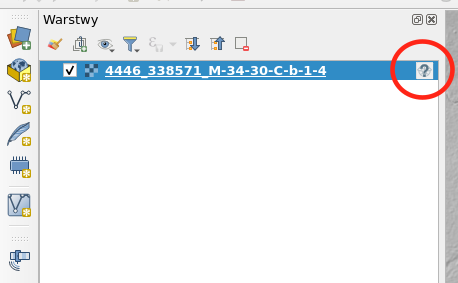
\includegraphics[width=10cm]{crs-cwiczenie1-brak-crs}
			\caption{Ostrzeżenie o braku zdefiniowanego CRS}
		\end{figure} 
	Po najechaniu na ten symbol i kliknięciu otworzy się nam okno \textbf{Wybór układu współrzędnych}. W polu filtra możemy szybko odszukać potrzebny nam układ - w tym wypadku \emph{ETRS89 / Poland CS92} o kodzie EPSG:2180. Po zatwierdzeniu \emph{OK} wracamy do głównego okna mapy.
	\begin{figure}[!ht]
    	\centering
	    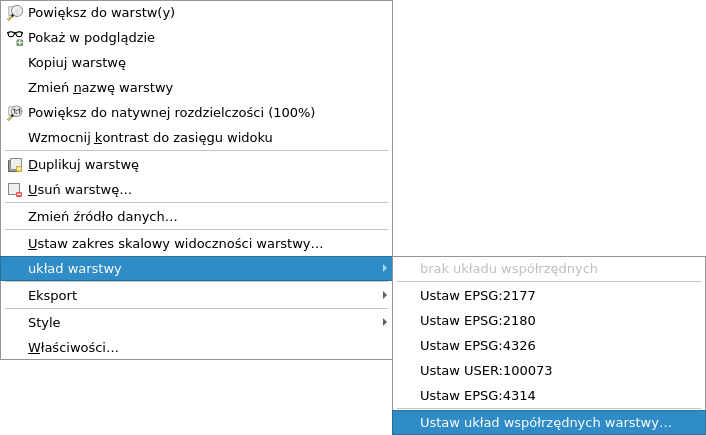
\includegraphics[width=10cm]{crs-cwiczenie1-menu-kontekstowe}
    	\caption{Menu kontekstowe warstwy - Ustawienie CRS}
    \end{figure} 
		\subsection{Zmiana odwzorowania rastra}
				W kolejnym ćwiczeniu zmienimy odwzorowanie naszej warstwy rastrowej i zapiszemy nowy zbiór na dysku.
		Wykorzystamy uprzednio otwarty raster NMT. Nasze zadanie możemy wykonać na dwa sposoby. Pierwszym jest wykorzystanie algorytmu processingu \textbf{Zmień odwzorowanie}. Ukaże się nam okno algorytmu, w którym wskazujemy kolejno:
		\begin{enumerate}
			\item warstwę wejściową
			\item źródłowy układ współrzędnych
			\item docelowy układ współrzędnych
			\item metodę resamplingu
			\item możliwe jest zdefiniowanie wartości NODATA
			\item dodatkowe parametry GDAL (np. kafelkowanie, typ kompresji)
			\item czy warstwa wyjściowa ma być zapisana na dysk, czy tylko wyświetlona jako tymczasowa
		\end{enumerate}
		\begin{figure}[!ht]
		\centering
		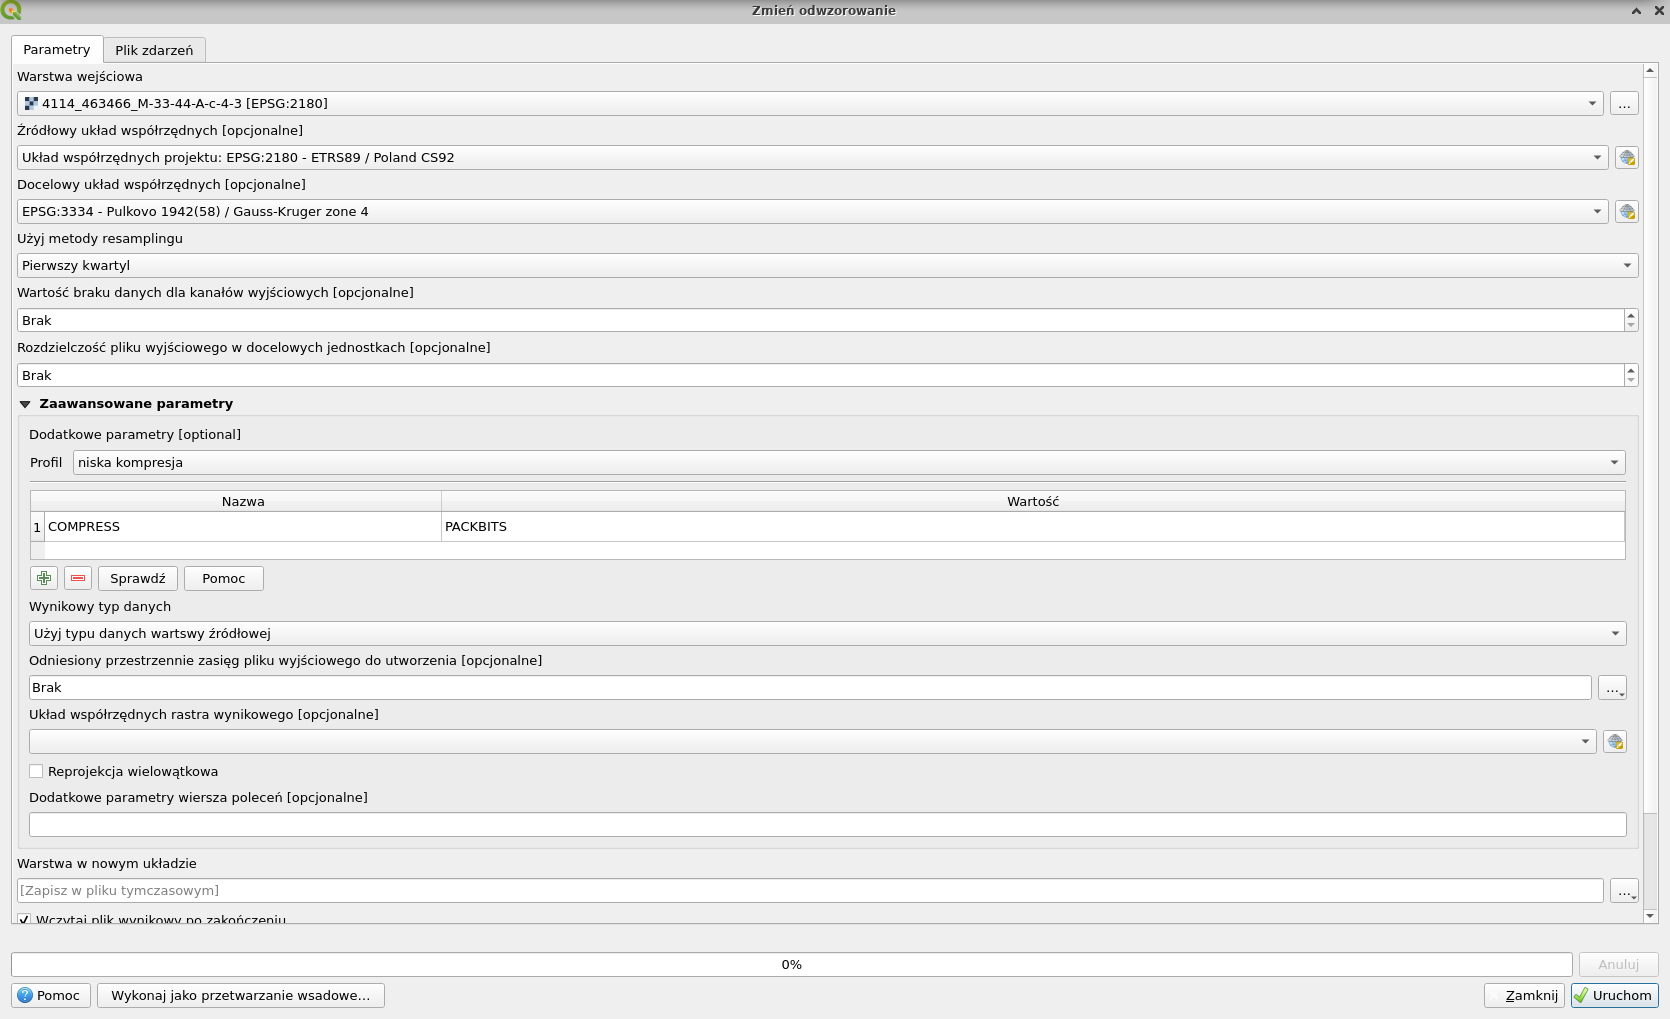
\includegraphics[width=10cm]{crs-cwiczenie2-zmien}
		\caption{Zmiana odwzorowania rastra}
	\end{figure} 
		Po zatwierdzeniu następuje transformacja rastra, która zależnie od jego wielkości może potrwać nawet kilkadziesiąt sekund.
		Druga metodą polega na zapisaniu istniejącej warstwy przy pomocy menu kontekstowego Eksport -> Zapisz Jako.
	\begin{figure}[!ht]
	\centering
	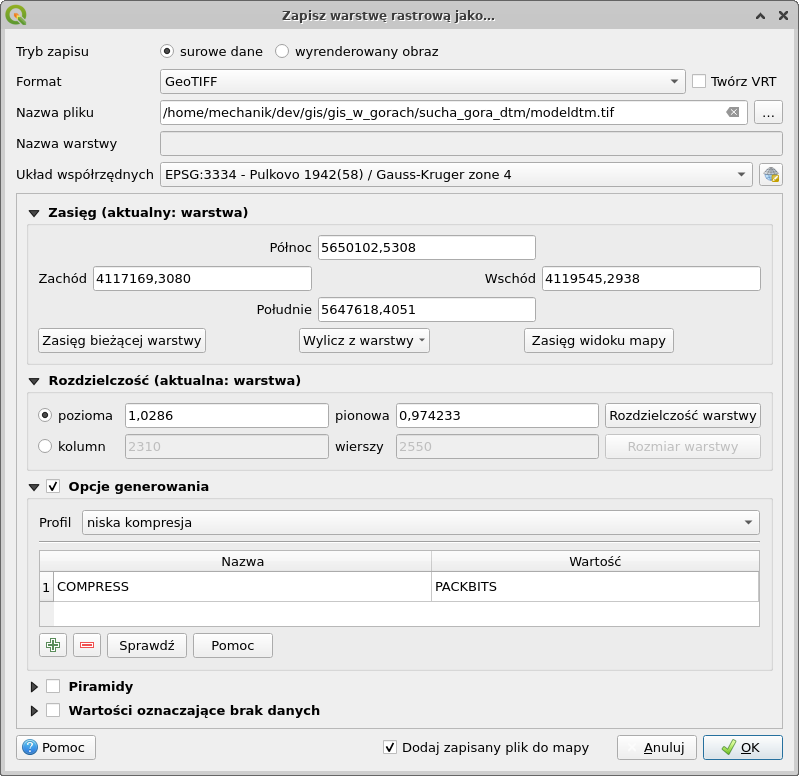
\includegraphics[width=10cm]{crs-cwiczenie2-zapisz-raster}
	\caption{Menu kontekstowe warstwy - Eksport Zapisz Jako}
\end{figure} 		
W tym wypadku również wskazujemy docelowy układ współrzędnych, ale także możemy wygodnie wskazać docelową rozdzielczość rastra.
	\subsection{Przypisanie układu współrzędnych wydruku}
	W ostatnim zadaniu tej sekcji przygotujemy arkusz wydruku mapy w odwzorowaniu azymutalnym Lamberta.
	\begin{enumerate}
		\item Zaczniemy w pustym projekcie, od załadowania zbioru \emph{/modul1/crs/prg/wojewodztwa.shp}. Są to granice województw pochodzące z Państwowego Rejestru Granic, w układzie współrzędnych 92.
		\item W kolejnym kroku uruchamiamy Menedżer wydruków i Nowy Wydruk (Ctrl+P)
		\begin{figure}[!ht]
			\centering
			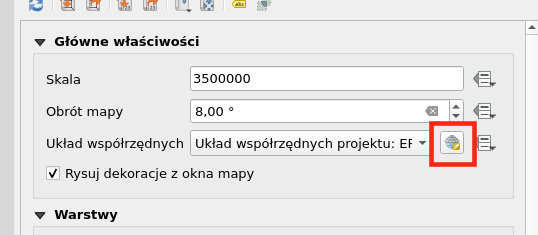
\includegraphics[width=5cm]{crs-wydruk-laea}
			\caption{Właściwości mapy - zmiana układu i skali}
		\end{figure}
		\item Na arkuszu osadzamy obiekt mapy, we właściwościach po prawej stronie ustawiamy skalę 1:3500000, oraz obrót 9 stopni, a następnie klikamy w symbol globusu poniżej (zobacz na ilustracji) i wskazujemy układ o symbolu EPSG:3035 (ETRS89-extended/LAEA Europe).
		\item W zakładce Siatka klikamy w ikonkę plusa, a następnie w przycisk Modyfikuj siatkę.
		\begin{figure}[!ht]
			\centering
			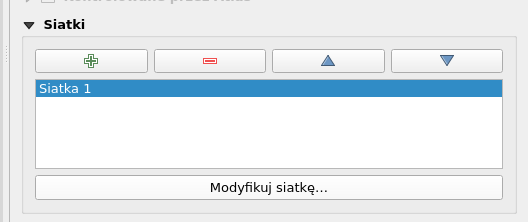
\includegraphics[width=5cm]{crs-laea-siatka}
			\caption{Zakładka Siatka - tworzenie nowej siatki kartograficznej}
		\end{figure}
		\item W ustawieniach Siatki (na ilustracji) wprowadzamy odstęp X i Y (wyrażony w jednostkach układu współrzędnych, tutaj metrach).
		\begin{figure}[!ht]
			\centering
			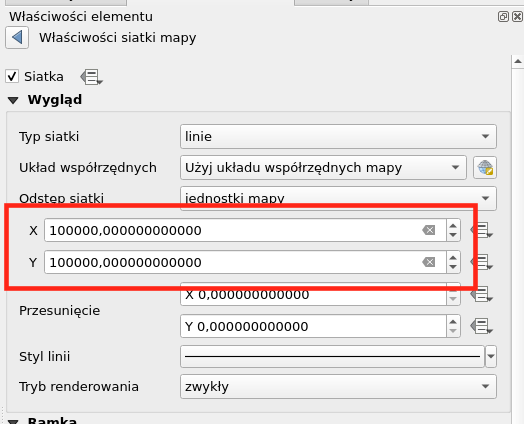
\includegraphics[width=5cm]{crs-laea-linie-siatki}
			\caption{Właściwości siatki}
		\end{figure}
		\item Na koniec zmieńmy odwzorowanie naszej mapy na stożkowe Lamberta (w oknie filtra wyboru układu użyjemy EPSG:3034, ETRS89-extended/LCC Europe), oraz skalę na 1:15000000, aby stwierdzić zniekształcenie linii południkowych.
	\end{enumerate} 

	\chapter{Praca z archiwalnymi rastrami}
		\section{Wprowadzenie}
			\begin{figure}[!ht]
			\centering
			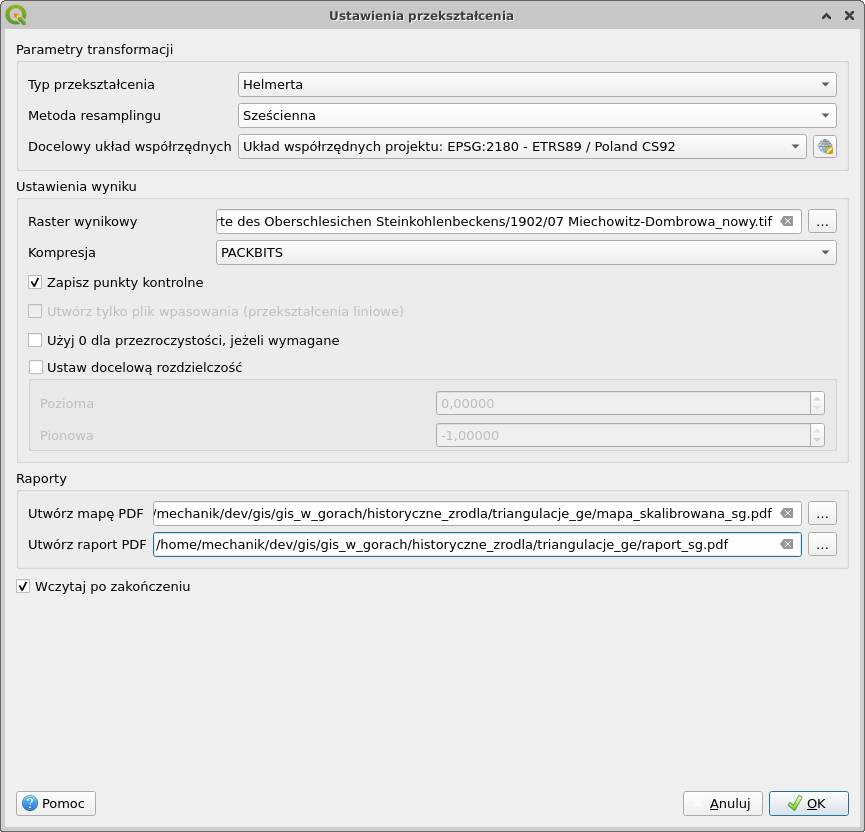
\includegraphics[width=10cm]{georef-ustawienia}
			\caption{Ustawienia Georeferencera}
		\end{figure} 
		\section{Referencja do punktów wspólnych}
		\begin{figure}[!ht]
			\centering
			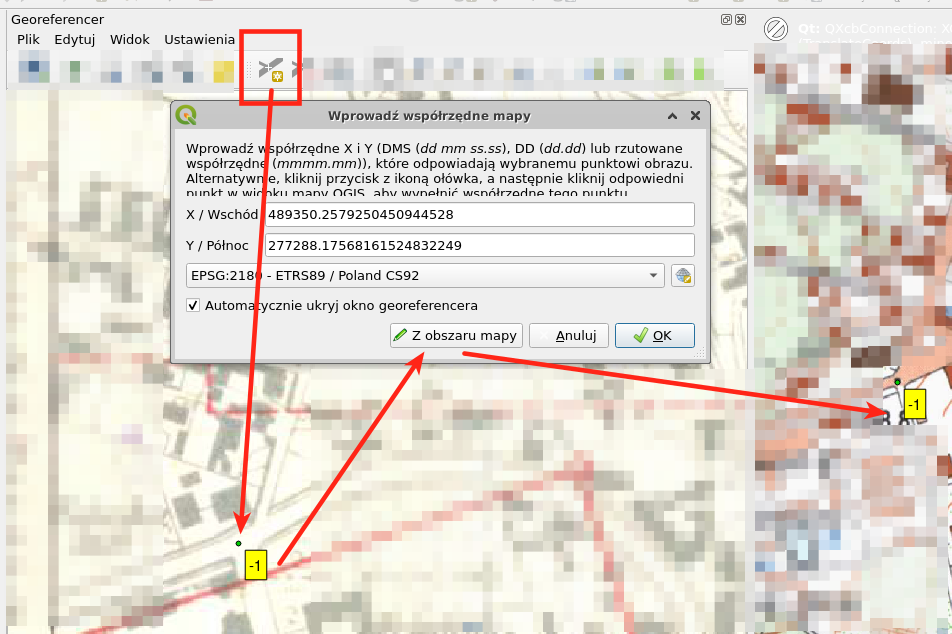
\includegraphics[width=10cm]{georef-dodaj}
			\caption{Dodawanie punktu}
		\end{figure}
		\begin{figure}[!ht]
		\centering
		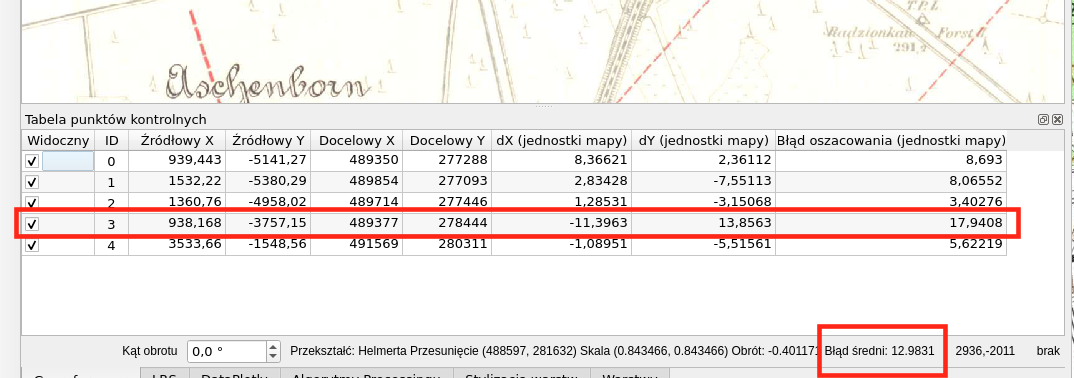
\includegraphics[width=10cm]{georef-tabela-punktow}
		\caption{Tabela punktów kontrolnych}
	\end{figure}  
		\section{Referencja do narożników mapy}
		\section{Ćwiczenia}

	\chapter{Referencja liniowa}
		\section{Wprowadzenie}
		\section{Przygotowanie zbioru liniowego}
		\section{Wyszukiwanie lokalizacji}
		\section{Ćwiczenia}

\part{Analiza}
	\chapter{Numeryczny model terenu - wprowadzenie}
		\section{Mapa spadków}
		\section{Mapa ekspozycji}
		\section{Inne wskaźniki topograficzne}
		\section{Ćwiczenia}
			\subsection{Wyznaczenie strefy narażonej osuwiskowo}
			\subsection{Stok narciarski}
	Wyszukanie stoku o ekspozycji północnej oraz nachylonego 10-30 stopni, wykorzystanie fuzzy logic
	\chapter{Widocznosc obiektów}
\section{Dominanty krajobrazu}
\section{Osie widokowe}
\section{Ćwiczenia}

\chapter{Nasłonecznienie}
\section{Mapa nasłonecznienia}
\section{Zmiana warunków}
\section{Potencjał solarny}
\section{Ćwiczenia}
\subsection{Strefy cienia}
\subsection{Jakość powierzchni dachowych dla fotowoltaiki}

\chapter{Wskaźniki urbanizacyjne}
\section{Powierzchnia zabudowy}
\section{Wskaźnik intensywności zabudowy}
\section{Powierzchnia biologicznie czynna}
\section{Ćwiczenia}
\subsection{Wyliczanie powierzchni zabudowy}

\chapter{Publikacja w internecie}
\section{GeoPDF}
\section{Strona html z osadzoną mapą}
\section{Geoportal Lizmap/QWC}
\section{Usługi w chmurze}
\section{Ćwiczenia}
\subsection{Nowa droga rowerowa}
\subsection{Plan zagospodarowania} 
\backmatter	

\tableofcontents*
\clearpage
%%% BIBLIOGRAPHY
%%% -------------------------------------------------------------

\bibliographystyle{abbrvnat}
\bibliography{qgis}

\end{document}